\chapter{Teoretické základy použitých algoritmů}
\label{chp: algos}
Za účelem zvýšení přesnosti identifikace aplikací, a~tedy zúžení kandidátní množiny generované pomocí metod \textit{JA3} či \textit{JA4}, je využit algoritmus pro~vyhledávání frekventovaných vzorů těchto otisků v~kontextu okolních \textit{TLS} spojení. Tato kapitola obsahuje obecný přehled algoritmů pro~vyhledávání frekventovaných vzorů, se zvláštním zaměřením na~princip a~využití algoritmu \textit{Apriori} a~jeho optimalizace.

Důvodem volby algoritmu \textit{Apriori} je jeho schopnost efektivně nacházet časté vzory v~transakčních datech, což lze analogicky aplikovat na~otisky \textit{TLS} spojení. Tento přístup umožňuje identifikovat opakující se kombinace otisků, které jsou charakteristické pro~specifické aplikace, a~tím efektivně eliminovat kandidáty, jejichž otisky s~těmito vzory nekorespondují.

\section{Algoritmy vyhledávající frekventované vzory}
Rozpoznávání frekventovaných vzorů v~datech představuje klíčovou a~nedílnou součást procesu dolování dat (\textit{data mining}). Tento krok umožňuje identifikovat opakující se vzory a~vztahy v~rozsáhlých datových souborech, které by jinak zůstaly skryté. V~rámci dolování dat se frekventované vzory využívají například pro~tvorbu asociačních pravidel, klasifikaci či shlukování. 

Typickými příklady využití jsou:
\begin{itemize}
	\item \textbf{Analýza nákupního chování zákazníků}, kde transakce představují množiny položek, které se společně vyskytují v~rámci nákupního chování~\cite{Aggarwal2014}.
	          
	\item \textbf{Analýza webových dat}, při~které se vyhledávají frekventované vzory ve~webových záznamech. Tyto vzory lze následně využít k~návrhu či vylepšení uživatelského rozhraní nebo ke~zlepšení personalizace obsahu~\cite{WebMining}. 
	          
	\item \textbf{Analýza softwarových chyb}, kde lze běh softwarových programů reprezentovat pomocí grafů obsahujících typické vzory. Logické chyby se často projevují jako specifické vzory, které je možné dále těžit pro~účely ladění a~diagnostiky~\cite{swBugs}.
\end{itemize}

Většina algoritmů pro~hledání frekventovaných vzorů je navržena v~rámci tradičního modelu založeného na~podpoře (\textit{support}) a~důvěře (\textit{confidence}). Existují však i~specializované přístupy, které využívají pokročilejší míry zajímavosti, modelují záporná pravidla nebo pracují s~omezeními pro~nalezení relevantnějších vzorů~\cite{Aggarwal2014}. Tato práce je zaměřena především na~algoritmus \textit{Apriori}, který je založen na~přístupu využívajícím podporu a~důvěru.

\section{Základní pojmy a~notace}
Před popisem samotného algoritmu \textit{Apriori} je vhodné uvést základní pojmy a~notace, které se v~oblasti dolování častých vzorů a~asociativních pravidel běžně používají.

\subsection{Transakce, položky a~jejich množiny}
Nechť množina položek \( I~= \{i_1, i_2, i_3, \dots, i_n\} \) reprezentuje například zboží v~obchodě či \textit{JA3/4} otisky \textit{TLS} spojení. Transakce \( T~\) je podmnožinou těchto položek, tedy \( T~\subseteq I~\). Množina všech transakcí tvoří transakční databázi \( D~= \{ T_1, T_2, T_3, \dots, T_m \} \). Množina položek (angl. \textit{itemset}) je libovolná kombinace prvků z~množiny \( I~\). Pokud množina položek (\textit{itemset}) obsahuje právě \( k~\) položek, nazýváme jej \textit{k-itemset}.

Množina častých položek (angl. \textit{frequent itemset}) je taková množina položek, která se v~transakční databázi vyskytuje alespoň s~minimální zadanou četností, zvanou podpora (\textit{support}). Míra \textit{podpory} (\textit{support}) je klíčovým kritériem pro~určení toho, zda je daná množina položek považována za~častou. 
Podpora množiny položek vyjadřuje, v~kolika transakcích z~celé databáze se daná množina vyskytuje. 
Formálně je definována jako:

\[
\text{support}(X) = \frac{\text{počet transakcí obsahujících } X}{\text{celkový počet transakcí}}
\]

Kandidátní množiny, jejichž podpora nedosahuje zvoleného prahu \textit{minsup} (minimální podpora), jsou z~dalšího zpracování vyřazeny.


\section{Algoritmus Apriori}
\textit{Apriori} je algoritmus určený pro~těžbu častých vzorců a~generování asociativních pravidel v~transakční databázích. Postupuje tak, že nejprve identifikuje časté jednotlivé položky v~databázi a~následně je rozšiřuje na~větší množiny, dokud se tyto množiny objevují v~databázi dostatečně často. Tyto časté vzory mohou být poté použity pro~generování asociativních pravidel, která reprezentují trendy a~závislosti v~databázi.

Algoritmus využívá přístup shora dolů pro~generování kandidátů, přičemž kandidáti jsou postupně rozšiřováni o~jednotlivé prvky. Skupiny kandidátů jsou následně ověřovány vůči databázi. Při~prohledávání se používá prohledávání do~šířky. Pro~efektivní počítání kandidátních množin je použita struktura hash stromu. Kandidátní množiny položek délky \(k\) se nejprve vytvoří na~základě množin častých položek délky \(k - 1\). Jsou odstraněny položky, které neobsahují podmnožinu s~častými položkami, a~prohledá se databáze transakcí, aby se mezi~zbývajícími kandidáty určily skutečné množiny frekventovaných položek~\cite{Agrawal1994}. Postup algoritmu \textit{Apriori} lze stručně shrnout pomocí následujícího pseudokódu, jenž byl převzat z~\cite{Agrawal1994}.

\begin{algorithm}[H]
\caption{Apriori algoritmus}
\SetKwInOut{Input}{Vstup}
\SetKwInOut{Output}{Výstup}
\Input{Transakční databáze $D$, Práh minimální podpory $minsup$}
\Output{Množina častých položek $L$}
$L_1 \gets$ všechny časté množiny délky 1 v~$D$\;
$k \gets 2$\;
\While{$L_{k-1} \ne \emptyset$}{
    $C_k \gets$ kandidátní množiny položek délky $k$ vygenerované z~$L_{k-1}$\;
    \ForEach{transakce $t \in D$}{
        \ForEach{kandidát $c \in C_k$}{
            \If{$c \subseteq t$}{
                zvýšit počet výskytů kandidáta $c$\;
            }
        }
    }
    $L_k \gets \{c \in C_k \mid support(c) \ge minsup\}$\;
    $k \gets k~+ 1$\;
}
\Return{$\bigcup_k L_k$}\;
\end{algorithm}

Výhodou algoritmu \textit{Apriori} je jeho systematický přístup založený na~teorii množin. 
Nevýhodou je však značná výpočetní náročnost při~práci s~velkým množstvím transakcí nebo položek, zejména při~generování velkého počtu kandidátních množin.

\subsection{Optimalizace algoritmu Apriori}
\label{subssec:optiApriori}
Hlavní nevýhodou algoritmu \textit{Apriori} je jeho vysoká výpočetní náročnost při~generování a~vyhodnocování kandidátních množin, zejména v~rozsáhlých transakčních databázích. Tento problém se projevuje zejména při~práci s~dlouhými množinami (\textit{itemsets}) a~vysokým počtem unikátních položek (\textit{unique items}), kdy počet potenciálních kombinací roste exponenciálně. V~extrémních případech může generování všech možných kombinací položek vést k~obrovskému množství kandidátů, z~nichž většina se nakonec neukáže jako častá. Tento jev, známý jako kandidátní exploze (\textit{candidate explosion}), významně zatěžuje paměťové i~výpočetní zdroje a~představuje hlavní slabinu algoritmu \textit{Apriori}~\cite{Agrawal1994}.

Za účelem omezení výpočetní zátěže bylo navrženo několik optimalizačních technik, které se snaží snížit počet generovaných kandidátních množin (\textit{candidate itemsets}). 

Následující nejvýznamnější strategie jsou převzaty z~\cite{HanAprioriOpti2012}:
\subsubsection{Počítání výskytů kandidátů s~využitím hašování } 
Strategie založená na~hašování množin položek do~odpovídajících bloků může být použita k~omezení velikosti kandidátních množin položek \( C_k \) pro~\( k~> 1 \). Při~procházení každé transakce v~databázi za~účelem generování častých 1-položkových množin je možné vygenerovat všechny 2-položkové kombinace položek pro~danou transakci a~namapovat je do~odpovídajících bloků v~hašovací tabulce, čímž se zvýší počet výskytů v~daném bloku.

2-položková množina, která má v~příslušném bloku počet výskytů nižší než je prahová hodnota podpory, nemůže být častá a~může být proto odstraněna z~kandidátní množiny. Tato strategie může výrazně snížit počet položkových množin, které je třeba následně vyhodnocovat (zejména v~případě, kdy \( k~= 2 \)).

\subsubsection{Redukce transakcí}
Redukce transakcí  spočívá ve~snížení počtu transakcí, které je nutné prohledávat v~následujících iteracích. Transakce, která neobsahuje žádnou častou množinu položek o~velikosti k~(angl. \textit{frequent k-itemset}), nemůže obsahovat ani žádnou častou množinu položek o~velikosti \( k~+ 1 \). Takovou transakci je tedy možné zcela vyřadit, neboť při~dalším průchodu databází při~hledání množin častých položek o~velikosti \( j~\), kde \( j~> k\), již nebude relevantní.


\subsubsection{Rozdělení (partitioning dat)}  
Technika rozdělení může být využita ke~zjištění množin častých položek při~dvou průchodech databází. Skládá se ze dvou fází, které jsou znázorněny na~diagramu~\ref{fig:partitioning_diagram}.

\begin{figure}[H]
	\centering
	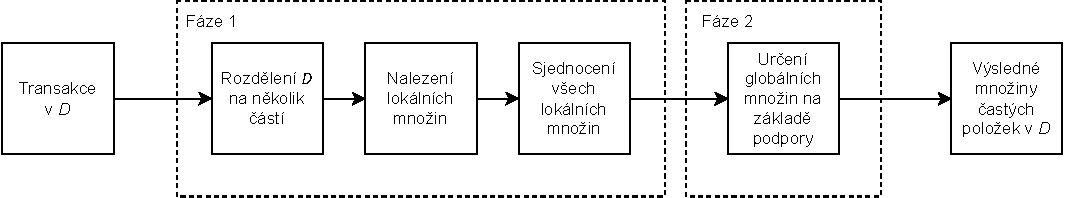
\includegraphics[width=\textwidth]{obrazky-figures/AproiriPart.drawio-crop.pdf}
    \caption{Ilustrace principu techniky rozdělení (partitioning), převzat z~\cite{HanAprioriOpti2012}}
    \label{fig:partitioning_diagram}
\end{figure}


\begin{enumerate}
    \item \textbf{Fáze I:} Databáze je rozdělena do~\( n~\) nepřekrývajících se částí (partitions). Pro~každou z~těchto částí se vypočítá nový lokální práh minimální podpory, definovaný jako \textit{minsup} \(\times\) počet transakcí v~dané části databáze. Dále se pro~každou část nalezne lokální množina častých položek.

    Lokální množina častých položek může, ale nemusí být častá s~ohledem na~celou databázi \( D~\). Nicméně každá množina, která může být potenciálně častá v~celé databázi, se musí vyskytnout jako častá alespoň v~jedné z~částí. Sjednocením častých množin ze všech částí vznikne globální množina kandidátů vůči databázi \( D~\).

    \item \textbf{Fáze II:} Proběhne druhý průchod databází \( D~\), při~kterém je pro~každou kandidátní množinu spočítána její skutečná podpora (\textit{support}) s~cílem určit globálně časté množiny položek. Velikost částí a~jejich počet jsou voleny tak, aby se každá část vešla do~hlavní paměti a~bylo ji možné načíst pouze jednou v~každé fázi.
\end{enumerate}
